\documentclass[Screen16to9,17pt]{foils}
\usepackage{zencurity-slides}

\externaldocument{basic-tcpip-and-security-exercises}
\selectlanguage{english}

\begin{document}

% # Praktisk introduktion til TCP/IP, netværk med sikkerhed og IPv6 (18.11)


% Netværk og TCP/IP for begyndere – Workshop I
% En hands-on workshop med fokus på netværksbegreber for begyndere

% Få styr på fundamentet bag al internettrafik – én gang for alle
% Uanset om du arbejder med udvikling, drift, support eller sikkerhed, så bygger alt på ét grundlag: netværket. TCP/IP
% er sproget, som får computere, servere og tjenester til at tale sammen, men hvad betyder det egentlig i praksis? På
% dette kursus får du en klar og praktisk introduktion til, hvordan netværk hænger sammen. Vi pakker de tekniske
% begreber ud, viser hvordan data bevæger sig på tværs af kabler og routere. Og du lærer selv at opsætte et netværk fra
% bunden.
%
% Gennem korte oplæg og praktiske øvelser lærer du at:

%   *   forstå og arbejde med IP-adresser
%   *   kende forskel på og bruge netkort, switch, og en router
%   *   konfigurere en moderne router via webinterface
%   *   se, hvordan routing fungerer på internettet
%   *   arbejde hands-on med netværk i praksis, både fælles og egne

% Du bliver introduceret til de vigtigste grundlæggende protokoller:
%
%   *   ARP – Address Resolution Protocol
%   *   IP og ICMP – Internet Control Message Protocol
%   *   TCP – Transmission Control Protocol
%   *   UDP – User Datagram Protocol
%   *   DHCP – Dynamic Host Configuration Protocol
%   *   DNS – Domain Name System
%
% Kurset ser på IPv4 og IPv6 side om side, så du forstår både paralleller og forskelle.
%
% Efter kurset vil du kunne:
%
%   *   opsætte og fejlfinde et lille netværk hjemme eller i en mindre virksomhed
%   *   forstå hvordan internettet “taler sammen”
%   *   læse netværkstrafik med fx Wireshark
%   *   arbejde mere sikkert og effektivt i dit daglige it-arbejde
%
% Praktisk info
% Medbring en computer (uanset styresystem) og en browser – mere skal der ikke til.
% Ingen forudgående kendskab til netværk eller TCP/IP kræves.
%
% Anbefalet bog men det er ikke et krav at købe denne:
% Practical Packet Analysis – Using Wireshark to Solve Real-World Network Problems
% 3rd edition (2017), Chris Sanders. ISBN: 9781593278021
% Nøgleord: TCP/IP, TCP, UDP, DHCP, DNS, ICMP

\mytitlepage
{Networking and TCP/IP for Beginners\\\vskip 1mm Workshop I: Basics}
{PROSA November 2026}

\hlkprofiluk

\slide{Goals for today}

\hlkimage{6cm}{bornhack-camp-2024.jpg}

\begin{list2}
\item Introduce basic networking and TCP/IP terminology
\item Show various network configurations with common protocols
\item Describe basics of TCP/IP
\item Let you get some hands on with IP protocols
\item Connecting to networks bring security risks, sorry -- so we will introduce a little security at the end
\end{list2}

Photo is NWWC camp at BornHack 2024, next is BornHack July 21. to 28. 2027 \link{https://bornhack.dk}


\slide{Time schedule}

\hlkimage{4cm}{kame-noanime-small.png}

\begin{list1}
\item 17:00 - 18:15 -- Session 0: Introduction and basic network terms, small exercises
\item 18:15 - 18:45 -- Break
\item 18:45 - 19:30 -- Session 1: Diving deeper into networking and TCP/IP
\item 19:30 - 19:45 -- Break
\item 19:45 - 20:30 -- Session 2: Try out a more exercises, play with protocols, see devices
\item 20:30 - 21:00 -- Activating firewalls, Discussion and questions
\end{list1}

During the presentation, in breaks etc. please do connect to the network, play with TCP/IP, switches and routers.

\slide{Session 0: Introduction and basic network terms, small exercises}


\slide{Exercises are completely optional}

We will use a combination of your systems, my networking hardware and my systems.\\
{\color{red} \bf There might be live sniffing done on traffic!}

We try to mimic what you would do in your own networks during the exercises.

\begin{list2}
\item Try ping and traceroute
\item See your own IP settings
\item Borrow a USB Ethernet and connect to a switch or router
\item Borrow a router home -- only brought a few!
\end{list2}

\slide{Linux is a toolbox}

I will use Linux and participants are welcome to use any operating system of their choice.

Note: even though I talk a lot about Unix, you can definitely run a lot of tools on Windows and Mac OS X.

\begin{list2}
\item Ping and traceroute - they are on every OS
\item USB Ethernet work on most operating system
\item USB Wi-Fi cards are fun, but some takes a little work to get going
\item Basic tools like the Nmap suite is available for Microsoft Windows, Mac OS X, Linux and many others
\end{list2}

Command line tools are sometimes used in the slides, as they only show text where a GUI screenshot can be cluttered with a lot of information, feel free to find GUI tools and web sites with same functionality



\slide{Prerequisites}

\textbf{\LARGE If you are interested in TCP/IP you are welcome}

\vskip 1cm
\begin{list1}
\item It is recommended to use virtual machines for the exercises
\item Network security and most internet related security work has the following requirements:
\begin{list2}
\item Network experience
\item TCP/IP principles - often in more detail than a common user
\item Programming is an advantage, for automating things
\item Some Linux and Unix knowledge is in my opinion a {\bf necessary skill} for infosec work\\
-- too many new tools to ignore, and lots found at sites like Github and Open Source written for Linux
\end{list2}
\end{list1}




\slide{Course Materials}

\begin{list2}
\item This material is in multiple parts:

\item Slide show - presentation - this file
\item Exercises - PDF which is used for this and other workshops
\item Additional resources from the internet are linked throughout
\item Wikipedia has a LOT of nice pages about IP protocols, for example:
\end{list2}

\begin{quote}\small
Transport Layer Security (TLS) is a cryptographic protocol designed to provide communications security over a computer network. The protocol is widely used in applications such as email, instant messaging, and voice over IP, but its use in securing HTTPS remains the most publicly visible.
\end{quote}
Source: \url{https://en.wikipedia.org/wiki/Transport_Layer_Security}

\slide{Book: Practical Packet Analysis (PPA)}


\hlkimage{6cm}{PracticalPacketAnalysis3E_cover.png}

\emph{Practical Packet Analysis,
Using Wireshark to Solve Real-World Network Problems}
by Chris Sanders, 3rd Edition
April 2017, 368 pp.
ISBN-13:
978-1-59327-802-1
\link{https://nostarch.com/packetanalysis3}

I recommend this book for people new to networking, it has been in HumbleBundle book bundles multiple times





\slide{Internet Today}

\begin{quote}
\textbf{\large Computer network}

In computer science, computer engineering, and telecommunications, \textbf{a network} is a \textbf{group} of communicating computers and peripherals called hosts, which communicate data to other hosts via communication protocols, as facilitated by networking hardware.

Within a computer network, \textbf{hosts} are identified by \textbf{network addresses}, which allow networking hardware to locate and identify hosts. Hosts may also have \textbf{hostnames}, memorable labels for the host nodes, which can be mapped to a network address using a hosts file or a name server such as \textbf{Domain Name Service}. The physical medium that supports information exchange includes \textbf{wired media like copper cables, optical fibers, and wireless radio-frequency media}. The arrangement of hosts and hardware within a network architecture is called the \textbf{network topology}.[1][2]


\end{quote}
Source: \url{https://en.wikipedia.org/wiki/Computer_network}


\slide{Course Network}
.
\hlkrightpic{65mm}{-1cm}{sample-network.png}

I have a course network with me which has the following information:
\begin{list2}
\item Routers -- computer with OpenBSD and portable routers
\item Switches and wireless access-points -- Unifi AP
\item Local LAN wired and wireless -- uses something called RFC1918 private addresses
\end{list2}

There is also a public network used in examples:
\begin{list2}
\item IPv4 addresses: 185.129.63.0/24 total 256, IPv6 addresses route6: 2a06:d380::/32
\item Autonomous system number: AS57860 Zencurity Aps\\
\url{https://en.wikipedia.org/wiki/Autonomous_system_(Internet)}
\end{list2}



\slide{Internet Today}

\hlkimage{13cm}{images/server-client.pdf}

\begin{list1}
\item Clients and servers, roots in the academic world
\item Protocols are old, very old! RFC 791: STD 5: Internet Protocol is from  September 1981!
\item Very few protocols were encrypted, today a lot has switched to HTTPS and TLS
\end{list1}

\slide{Internet is Open Standards!}

{\hlkbig \color{titlecolor}
We reject kings, presidents, and voting.\\
We believe in rough consensus and running code.\\
-- The IETF credo Dave Clark, 1992.}

\begin{list1}
\item Request for comments (RFC) -- a series of documents spanning decades
\item RFC, BCP, FYI, informational -- first ones from 1969!
\item Are not updated but status is changed to Obsoleted when new versions are published
\item Standards track:\\
Proposed Standard $\rightarrow$ Draft Standard $\rightarrow$ Standard
\end{list1}

\slide{Internetworking: history}

\begin{list2}
\item[1961]  L. Kleinrock, MIT packet-switching theory
\item[1962]  J. C. R. Licklider, MIT - notes
\item[1964]  Paul Baran: On Distributed Communications
\item[1969]  ARPANET 4 nodes
\item[1971]  14 nodes
\item[1973]  Design of Internet Protocols started
\item[1973]  Email is about 75\% of all ARPANET traffic
\item[1974]  TCP/IP: Cerf/Kahn: A protocol for Packet
        Network Interconnection
\item[1983]  EUUG $\rightarrow$ DKUUG/DIKU Denmark
\item[1988]  About 60.000 systems on the internet -
        The Morris Worm hits about 10\%
\item[2002] About 130 million Internet hosts
\item[2010] IANA reserved blocks 7\% (Maj 2010) - \link{http://www.potaroo.net/tools/ipv4/}
\end{list2}

\slide{Internet historically set -  anno 1969}
\hlkimage{6cm}{1969_4-node_map.png}
%size 2

\begin{list2}
\item Node 1: University of California Los Angeles
\item Node 2: Stanford Research Institute
\item Node 3: University of California Santa Barbara
\item Node 4: University of Utah
%\item Kilde: \link{http://www.zakon.org/robert/internet/timeline/}
\end{list2}

\slide{What are Internet hosts }

\vskip 1 cm

\centerline{World Wide Web servers}

\hlkimage{15cm}{images/Count_WWW.png}

\begin{list1}
\item Source: Hobbes' Internet Timeline v5.6
\link{http://www.zakon.org/robert/internet/timeline/}
\end{list1}

\slide{What are Internet hosts }

\hlkimage{15cm}{potaroo-ipv4-address-report.png}
\centerline{Cumulative RIR address assignments, per RIR}

\begin{list1}
\item Source:
IPv4 Address Report \link{http://www.potaroo.net/tools/ipv4/}
\end{list1}

\slide{What is the Internet}

\begin{list1}
\item Communication between humans - currently!
\item Based on TCP/IP
\begin{list2}
\item best effort -- send it off, hope for the best, often it is received at destination
\item packet switching (IPv6 calls it packets, not datagram)
\item \emph{connection-oriented} TCP
\item \emph{connection-less} UDP
\end{list2}
\end{list1}

RFC-1958:
\begin{quote}
 A good analogy for the development of the Internet is that of
 constantly renewing the individual streets and buildings of a city,
 rather than razing the city and rebuilding it. The architectural
 principles therefore aim to provide a framework for creating
 cooperation and standards, as a small "spanning set" of rules that
 generates a large, varied and evolving space of technology.
\end{quote}


\slide{What the internet is actually made up of}


\hlkimage{13cm}{how-the-internet-works.jpg}
{\small Source: \emph{How the Internet Really Works
An Illustrated Guide to protocols, privacy, censorship, and governance} by catnip and article 19}\\
\url{https://catnip.article19.org/} {\color{red}\faHeart}
fun and educational book


\slide{Network data at different layers}

\hlkimage{16cm}{sample-ip-network.pdf}


\begin{list2}
\item Network traffic is sent using network protocols with fields, values and destinations
\item Can we inspect this and decide to pass or block traffic, certainly! Does it help, sure!
\end{list2}


\slide{Protocols: OSI and Internet models}

\hlkimage{9cm,angle=90}{images/compare-osi-ip.pdf}

Protocols are rules, like how to say; Hello!
Don't worry too much yet, this is an overview!


\slide{Recommended network technologies to learn}

Small set of recommended networking technologies to learn

Networking: Basic Protocols from the Internet Protocols suite -- TCP/IP
\begin{list2}
\item Network Layer: Ethernet, Address Resolution Protocol (ARP), IPv4 and ICMPv4
\item Transport Layer: Transmission Control Protocol (TCP) and User Datagram Protocol (UDP)
\item Common upper layer: Dynamic Host Configuration Protocol (DHCP), Domain Name System (DNS),
Hypertext Transfer Protocol (HTTP)\\
\vskip 5mm
\item Later add the encrypted/secure versions like Hypertext Transfer Protocol Secure (HTTPS) which uses Transport Layer Security (TLS)
\item Later add Wi-Fi and IPv6/ICMPv6 with Neighbor Discovery Protocol (NDP)
\end{list2}

Enough to be able to go to other resources, and a connected path from ARP to TLS



\slide{How to use the Internet Protocols (IP) with DNS}

Names are used by humans when browsing, sending email etc.

\hlkimage{15cm}{garden-small-screenshot.png}

\slide{The Domain Name System (DNS)}

Names are used by humans
\begin{center}
www.kramse.org   hlk@kramse.org
\end{center}

Computers use the addresses
\begin{alltt}
$ host www.kramse.dk
www.kramse.dk has address 185.129.63.130
www.kramse.dk has IPv6 address 2a06:d380:0:102::80
...
mail.kramse.org has address 185.129.63.250
mail.kramse.org has IPv6 address 2a06:d380:0:102::25
\end{alltt}

This is the main feature of Domain Name System (DNS) -- forward and reverse lookups\\
See more at \link{https://en.wikipedia.org/wiki/Domain_Name_System}


\slide{IPv4 ran out of addresses}

\hlkimage{10cm}{ipv4-address-report-potaroo-plotend.png}
Source: \link{http://www.potaroo.net/tools/ipv4/}

We have essentially run out of IPv4 public addresses, so almost everyone uses Network Address Translation (NAT)


\slide{Common Address Space}

\vskip 2 cm
\hlkimage{13cm}{IP-address.pdf}

\begin{list2}
\item Internet is defined by the address space
\item IPv4 based on 32-bit addresses, example \textbf{dotted decimal} format 10.0.0.1
\item IPv6 very similar to IPv4 without NAT, 128-bit addresses in hex ::1, 2a06:d380:0:101::80
\end{list2}


\slide{Internet ABC was replaced by CIDR}

\hlkimage{15cm}{CIDR-aggregation.pdf}

\begin{list2}
\item Previously we used classes: A, B, C, D og E
See \link{http://en.wikipedia.org/wiki/Classful\_network}
\item This proved to be a bit inflexible and today we use CIDR
\item Classless Inter-Domain Routing (CIDR) always use subnet mask which is a number of 1-bit followed by zeroes
\item 10.0.0.0/24 means the network 10.0.0.0 with 24 subnet bits (mask 255.255.255.0)
\item 2a06:d380:0:101::80/64 means the network with 64-bit prefix length
\item \textbf{Supernet} is when more networks are \textbf{aggregated} into one
\end{list2}

\slide{RFC-1918 Private Networks}


Address Allocation for Private Internets RFC-1918
\begin{list2}
\item 10.0.0.0    -  10.255.255.255  (10/8 prefix)
\item 172.16.0.0  -  172.31.255.255  (172.16/12 prefix)
\item 192.168.0.0 -  192.168.255.255 (192.168/16 prefix)
\end{list2}

Can be used by anyone in their own local area network (LAN)

A typical \emph{home network} would use 192.168.0.0/24 with 192.168.0.1 being the router


\slide{Documentation Prefix, IPv6 updates etc.}

Even documentation has its own prefix, RFC5737:
\begin{alltt}
The blocks 192.0.2.0/24 (TEST-NET-1), 198.51.100.0/24 (TEST-NET-2),
and 203.0.113.0/24 (TEST-NET-3) are provided for use in
documentation.
\end{alltt}

IPv6 listed in RFC3849 \verb+2001:DB8::/32+
with RFC 9637 (2024) added a larger documentation block, \verb+3fff::/20+



See RFC3330 \emph{Special-Use IPv4 Addresses} which is updated by
RFC6890 \emph{Special-Purpose IP Address Registries} which in turn is updated by RFC8190\\
Use the web version of RFCs to surf back and forth \link{https://www.rfc-editor.org/rfc/rfc8190}



\slide{Ethernet and Bridges}

\hlkimage{9cm}{ethernet73_large.png}
Original by Robert M. Metcalfe

\begin{list2}
\item Ethernet is a broadcast technology data transmitted into the ether -- a cable
\item This limits how many devices to connect, but using bridges we can connect segments\\
 -- which copy between them if needed
\item It learns the devices on each side (MAC address)
\item See also \link{http://en.wikipedia.org/wiki/ALOHAnet}
\end{list2}


\slide{Hardware addressing}
%\hlkimage{10cm}{apple-oui.png}

Many LAN hardware devices use \emph{hardware address} -- MAC \textbf{a8:5e:45:bc:6b:f7}

\begin{alltt}
A8-5E-45   (hex)		ASUSTek COMPUTER INC. 27 July 2019
A85E45     (base 16)		ASUSTek COMPUTER INC.
				15,Li-Te Rd., Peitou, Taipei 112, Taiwan
				Taipei  Taiwan  112
				TW
\end{alltt}
\begin{list2}
\item Network technologies use a layer 2 hardware address
\item Typically using 48-bit Media Access Control (MAC) addresses known from Ethernet MAC-48/EUI-48
\item First half is assigned to companies -- Organizationally Unique Identifier (OUI)
\item Using the OUI you can see which producer and roughly when a network chip was produced
\item \link{http://standards.ieee.org/regauth/oui/index.shtml}
\end{list2}



\slide{Ethernet, cables}

\hlkimage{17cm}{ethernetLights.jpg}

\centerline{Show link, and activity -- blinkenlights}




\slide{A switch -- many bridges combined into one device}

\hlkimage{9cm}{switch-1.pdf}

\begin{list2}
\item Today we use switches, Don't buy a hub, not even for experimenting or sniffing
\item A switch can receive and send data on multiple ports at the same time in the \textbf{same subnet}
\item Performance only limited by the backplane and switching chips
\item Switches can often \textbf{route} with the same speed and mirror packets
\item \textbf{Routing connects subnets} -- moving packets between subnets
\end{list2}


\slide{Wireless }

\hlkimage{10cm}{WCG200v2_med.jpg}

\begin{list1}
\item A typical home router would have built-in 802.11 Access-Point (AP) and some Ethernet LAN ports
\end{list1}


\slide{Wifi network cards}

\hlkimage{10cm}{TL-WN722N.png}

\begin{list2}
\item Your devices typically have (multiple) wireless chips supporting wireless communication
\item Card shown is TP-link TL-WN722N hardware version 2.0 cheap but only support 2.4GHz
\item Alfa AWUS036ACH 2.4GHz + 5GHz Dual-Band and high performing
\item Both work great in Kali Linux for our purposes, {\bf but are older models by now}
\end{list2}

Unfortunately the vendors change models often enough that the above are hard to find. I recommend using your favourite search engine and research which cards work with Kali Linux and airodump-ng.

\slide{Wi-Fi Introduction and Security}

\begin{list1}
\item Wifi standards IEEE 802.11
\begin{list2}
\item 802.11b 11Mbps
\item 802.11g 54Mbps
\item 802.11n faster
\item 802.11i Security enhancements Robust Security Network RSN
\end{list2}
\item New names:\\
Wi-Fi 6 to identify devices that support 802.11ax technology\\
Wi-Fi 5 to identify devices that support 802.11ac technology\\
Wi-Fi 4 to identify devices that support 802.11n technology
\end{list1}

Source: \link{http://grouper.ieee.org/groups/802/11/index.html}



\slide{A modern router}

\hlkimage{7cm}{sft1200_1.png}

\begin{list2}
\item Opal (GL-SFT1200) is a pocket-sized travel router supporting 1200Mbps wireless,
Max. 300 Mbps (2.4GHz) + 867 Mbps (5GHz) Fast Wi-Fi Speeds, Powerful CPU with 3 x Gigabit Ports,
Excellent Security with VPN -- OpenVPN \& WireGuard, IPv6
\end{list2}
Source: \url{https://www.gl-inet.com/products/gl-sft1200/}


\slide{Topologier and Spanning Tree Protocol (STP)}

\hlkimage{13cm}{switch-STP.pdf}

See more in Radia Perlman, \emph{Interconnections: Bridges, Routers, Switches, and Internetworking Protocols}

\slide{Core, Distribution and Access net}

\hlkimage{17cm}{core-dist.pdf}

\centerline{Not always using these terms in modern networking}

\slide{Bridges and routers across a Wide Area Network (WAN)}

\hlkimage{17cm}{wan-network.pdf}

\slide{Packets of data -- postcards of the Internet}

\hlkimage{18cm}{ethernet-frame-1.pdf}
\begin{list1}
\item Looking deeper data is laid out according to a structure -- \textbf{frames and packets}
\item Often a start and end signal of a frame -- like Ethernet
\item Today we talk about packets of 1500 bytes which is common in Ethernet
\item Operating system masks a lot of complexity
\end{list1}




\slide{IPv4 header - RFC-791 september 1981}

\begin{alltt}\footnotesize
    0                   1                   2                   3
    0 1 2 3 4 5 6 7 8 9 0 1 2 3 4 5 6 7 8 9 0 1 2 3 4 5 6 7 8 9 0 1
   +-+-+-+-+-+-+-+-+-+-+-+-+-+-+-+-+-+-+-+-+-+-+-+-+-+-+-+-+-+-+-+-+
   |Version|  IHL  |Type of Service|          Total Length         |
   +-+-+-+-+-+-+-+-+-+-+-+-+-+-+-+-+-+-+-+-+-+-+-+-+-+-+-+-+-+-+-+-+
   |         Identification        |Flags|      Fragment Offset    |
   +-+-+-+-+-+-+-+-+-+-+-+-+-+-+-+-+-+-+-+-+-+-+-+-+-+-+-+-+-+-+-+-+
   |  Time to Live |    Protocol   |         Header Checksum       |
   +-+-+-+-+-+-+-+-+-+-+-+-+-+-+-+-+-+-+-+-+-+-+-+-+-+-+-+-+-+-+-+-+
   |                       Source Address                          |
   +-+-+-+-+-+-+-+-+-+-+-+-+-+-+-+-+-+-+-+-+-+-+-+-+-+-+-+-+-+-+-+-+
   |                    Destination Address                        |
   +-+-+-+-+-+-+-+-+-+-+-+-+-+-+-+-+-+-+-+-+-+-+-+-+-+-+-+-+-+-+-+-+
   |                    Options                    |    Padding    |
   +-+-+-+-+-+-+-+-+-+-+-+-+-+-+-+-+-+-+-+-+-+-+-+-+-+-+-+-+-+-+-+-+

                    Example Internet Datagram Header
\end{alltt}
Source: \url{https://datatracker.ietf.org/doc/html/rfc791} and updated later

\slide{IPv6 header - RFC-1883 December 1995}
\vskip -1cm
\begin{alltt}\footnotesize
   +-+-+-+-+-+-+-+-+-+-+-+-+-+-+-+-+-+-+-+-+-+-+-+-+-+-+-+-+-+-+-+-+
   |Version| Traffic Class |           Flow Label                  |
   +-+-+-+-+-+-+-+-+-+-+-+-+-+-+-+-+-+-+-+-+-+-+-+-+-+-+-+-+-+-+-+-+
   |         Payload Length        |  Next Header  |   Hop Limit   |
   +-+-+-+-+-+-+-+-+-+-+-+-+-+-+-+-+-+-+-+-+-+-+-+-+-+-+-+-+-+-+-+-+
   |                                                               |
   +                                                               +
   |                                                               |
   +                         Source Address                        +
   |                                                               |
   +                                                               +
   |                                                               |
   +-+-+-+-+-+-+-+-+-+-+-+-+-+-+-+-+-+-+-+-+-+-+-+-+-+-+-+-+-+-+-+-+
   |                                                               |
   +                                                               +
   |                                                               |
   +                      Destination Address                      +
   |                                                               |
   +                                                               +
   |                                                               |
   +-+-+-+-+-+-+-+-+-+-+-+-+-+-+-+-+-+-+-+-+-+-+-+-+-+-+-+-+-+-+-+-+
\end{alltt}
%Source: \url{https://datatracker.ietf.org/doc/html/rfc1883} and obsoleted by\\
%\url{https://datatracker.ietf.org/doc/html/rfc8200}



\slide{Windows - ipconfig}

\hlkimage{14cm}{win-ipconfig-ipv6.png}

\slide{Windows -- control panel with DHCP}
\hlkimage{10cm}{win-control-panel-ipv6.png}

DHCP is responsible for giving you a dynamic address



\slide{ Dynamic Host Configuration Protocol (DHCP)}

\hlkimage{10cm}{dhcp-1.pdf}

\begin{list1}
\item How does a system get the address?
\item Typically in  IPv4 they will get them from DHCP
\item System sends a DHCP request, server allocates an address \emph{lease}
\item IPv6 typically uses Router Advertisement -- get prefix, configure their own IPv6 address
\end{list1}



\slide{Unix - practical examples ifconfig and ping}

\begin{alltt}\small
$ ifconfig en0
en0: flags=8863<UP,BROADCAST,SMART,RUNNING,SIMPLEX,MULTICAST> mtu 1500
        inet6 {\bf fe80::216:cbff:feac:1d9f%en0} prefixlen 64 scopeid 0x4
        inet {\bf 10.0.42.15} netmask 0xffffff00 broadcast 10.0.42.255
        inet6 {\bf 2001:16d8:dd0f:cf0f:216:cbff:feac:1d9f} prefixlen 64 autoconf
        ether 00:16:cb:ac:1d:9f
        media: autoselect (1000baseT <full-duplex>) status: active

$ ping6 ::1
PING6(56=40+8+8 bytes) ::1 --> ::1
16 bytes from ::1, icmp_seq=0 hlim=64 time=0.089 ms
16 bytes from ::1, icmp_seq=1 hlim=64 time=0.155 ms

$ traceroute6 2001:16d8:dd0f:cf0f::1
traceroute6 to 2001:16d8:dd0f:cf0f::1 (2001:16d8:dd0f:cf0f::1)
from 2001:16d8:dd0f:cf0f:216:cbff:feac:1d9f, 64 hops max, 12 byte packets
 1  2001:16d8:dd0f:cf0f::1  0.399 ms  0.371 ms  0.294 ms
\end{alltt}


\slide{ICMP and Ping}

\begin{list1}
\item Internet Control Message Protocol (ICMP)
\item Error conditions are signalled using this
\item The ping program sends ICMP ECHO request and
 expect ICMP ECHO reply
\item
\begin{alltt}
\small {\bfseries
$ ping 192.168.1.1}
PING 192.168.1.1 (192.168.1.1): 56 data bytes
64 bytes from 192.168.1.1: icmp_seq=0 ttl=150 time=8.849 ms
64 bytes from 192.168.1.1: icmp_seq=1 ttl=150 time=0.588 ms
64 bytes from 192.168.1.1: icmp_seq=2 ttl=150 time=0.553 ms
\end{alltt}
\end{list1}

\slide{traceroute}

\begin{list1}
\item traceroute works using the Time to Live (TTL) or Hop-Count fields
\item Each router will subtract one from this, and if zero -- return ICMP message
\item Unix uses UDP with a high port number as destination, receives ICMP Port Unreachable
\item The tool is called \verb+tracert+ on Microsoft Windows and uses ICMP Echo request
\begin{alltt}
\small{\bfseries
$ traceroute 185.129.60.129}
traceroute to 185.129.60.129 (185.129.60.129),
30 hops max, 40 byte packets
 1  safri (10.0.0.11)  3.577 ms  0.565 ms  0.323 ms
 2  router (185.129.60.129)  1.481 ms  1.374 ms  1.261 ms
\end{alltt}
\end{list1}



\slide{NAT Network Address Translation}
\hlkimage{16cm}{nat-1.pdf}


\vskip 2 cm
\begin{list2}
\item NAT is used for connecting private networks to the Internet
\item NAT gateway replaces source address and forwards packets
\item A quick and dirty fix that keeps messing up networks and protocols
\item The NAT router/firewall has state tables
\end{list2}

\slide{ARP in IPv4}

\begin{center}
\colorbox{white}{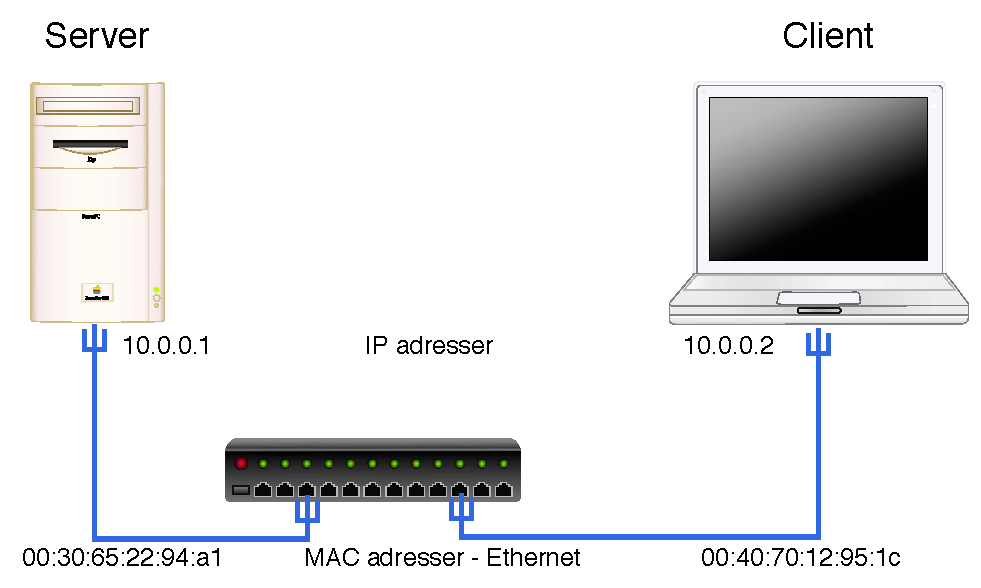
\includegraphics[width=18cm]{images/arp-basic.pdf}}
\end{center}

%server 00:30:65:22:94:a1\\
%client 00:40:70:12:95:1c\\
%hacker 00:02:03:04:05:06\\


\slide{ARP request and reply}
\begin{list1}
\item {\bfseries ping 10.0.0.2} from server
\item ARP Address Resolution Protocol request/reply:
  \begin{list2}
  \item ARP request broadcasted on layer 2 - Who has 10.0.0.2 Tell 10.0.0.1
  \item ARP reply (from 10.0.0.2) 10.0.0.2 is at 00:40:70:12:95:1c
  \end{list2}
\item IP ICMP request/reply:
  \begin{list2}
    \item Echo (ping) request from 10.0.0.1 to 10.0.0.2
\item Echo (ping) reply from 10.0.0.2 to 10.0.0.1
\item ...
  \end{list2}
\item ARP is performed on Ethernet before IP can be transmitted
\end{list1}


\exercise{ex:ping}
\exercise{ex:basic-dns-lookup}


\breakdance

\slide{Session 1: Diving deeper into networking and TCP/IP}


\slide{User Datagram Protocol (UDP)}
\hlkimage{16cm}{udp-1.pdf}
Connectionless \url{https://en.wikipedia.org/wiki/User_Datagram_Protocol}


\slide{Transmission Control Protocol (TCP)}
\hlkimage{14cm}{tcp-1.pdf}

Connection-oriented \url{https://en.wikipedia.org/wiki/Transmission_Control_Protocol}


\slide{TCP three way handshake}

\hlkimage{6cm}{images/tcp-three-way.pdf}

\begin{list2}
\item Session setup is used in some protocols
\item Other protocols like HTTP/2 can perform request in the first packet
\end{list2}


\slide{Well-Known Port Numbers}

\hlkimage{6cm}{iana1.jpg}

\begin{list1}
\item IANA maintains a list of magical numbers in TCP/IP
\item Lists of protocl numbers, port numers etc.
\item A few notable examples:
\begin{list2}
\item Port 25/tcp Simple Mail Transfer Protocol (SMTP)
\item Port 53/udp and 53/tcp Domain Name System (DNS)
\item Port 80/tcp Hyper Text Transfer Protocol (HTTP)
\item Port 443/tcp HTTP over TLS/SSL (HTTPS)
\end{list2}
\item Source: \link{http://www.iana.org}
\end{list1}


\slide{Whois -- Where do IP addresses come from}

\begin{list1}
\item A these magical numbers we use on the internet are administered by IANA \url{https://www.iana.org/}
\item They have handed out portions to the Region Internet Registries (RIR)
\begin{list2}
\item RIPE (Réseaux IP Européens)  \link{http://ripe.net}
\item ARIN American Registry for Internet Numbers \link{http://www.arin.net}
\item Asia Pacific Network Information Center \link{http://www.apnic.net}
\item LACNIC (Regional Latin-American and Caribbean IP Address Registry) - Latin America and some Caribbean Islands
\end{list2}
\item AFRINIC \url{https://afrinic.net/}
\item They are memberbased, and members are called Local Internet Registries (LIRs) og National Internet Registry (NIR)
\end{list1}



\slide{Hosting and internet providers}

\hlkimage{16cm}{network-bgp-asn.png}

\begin{list2}
\item BGP networks are used for all of the Internet
\item New standards like Resource Public Key Infrastructure (RPKI) are underway
\item Try RIPE BGPlay \url{https://stat.ripe.net/special/bgplay#bgplay_fetch.resource=185.129.60.1}
\end{list2}


\slide{Routing Basics: Prefixes, AS and BGP}

\begin{list2}
\item {\bf Prefix} -- a block of addresses, like 192.0.2.0/24 or 2001:db8:1234::/48
\item {\bf Autonomous System (AS)} -- a network under one routing policy, identified by an AS number (ASN) registered at an RIR such as RIPE NCC
\item {\bf BGP} -- Border Gateway Protocol, how autonomous systems tell each other which prefixes they can reach
\item {\bf RPKI and ROA} -- signed statements of which AS may originate a prefix, prefixes without a valid ROA are filtered by many networks
\item {\bf Upstream / transit} -- the provider that announces your prefixes to the rest of the internet
\item {\bf Smallest routable prefix} -- normally /24 for IPv4 and /48 for IPv6
\item Using your own PI addresses requires an ASN, a BGP session and an upstream willing to announce them -- usually a business connection.
\item Exception: Netnørden offers BGP on private connections \link{https://netnoerden.dk/faq}
\end{list2}


\slide{Public IP address: Provider Aggregatable (PA) Addresses}

\begin{quote}
PA addresses are assigned from an LIR's allocation and are registered in the RIPE Database
by the LIR. The advantage of PA addresses is that the routing information for many customers
can be aggregated once it leaves the provider's routing domain.
\end{quote}
Source: RIPE Network Coordination Centre (RIPE NCC) -- FAQ: ISPs\\
\link{https://www.ripe.net/membership/member-support/faqs/isp-related-questions/pa-pi/}

\begin{list2}
\item Assigned from a Local Internet Registry's (LIR) own allocation
\item Registered in the RIPE Database by the LIR itself
\item Routing information for many customers can be {\bf aggregated} into a single announcement, improving global routing efficiency
\item If an end user changes their upstream provider, the PA addresses {\bf must be returned} -- they cannot be taken along
\item {\bf Usually one IPv4 for your router, or shared NAT (CGNAT) -- you are here}
\end{list2}

\slide{Public IP address: Provider Independent (PI) Addresses}

\begin{quote}
PI address space is assigned separately and not from an LIR's PA allocation. All PI
assignments are registered in the RIPE Database by the RIPE NCC at the time they are
assigned. PI assignments are usually small; they cannot be aggregated into larger blocks.
The disadvantage of this is that network operators throughout the Internet may choose
not to route them.
\end{quote}
Source: RIPE Network Coordination Centre (RIPE NCC) -- FAQ: ISPs\\
\link{https://www.ripe.net/membership/member-support/faqs/isp-related-questions/pa-pi/}

\begin{list2}
  \item Assigned {\bf directly by the RIPE NCC} (a Regional Internet Registry),
        not from an LIR's allocation
  \item Registered in the RIPE Database by the RIPE NCC at assignment time
  \item Usually small blocks that {\bf cannot be aggregated} into larger ones
  \item The end user {\bf retains} the address block even when changing ISPs
  \item Network operators across the Internet may choose {\bf not to route} PI
        assignments due to lack of aggregation
\end{list2}

\slide{Current Status IP addresses IPv4 vs IPv6}

\begin{quote}
As the RIPE NCC has run out of IPv4 addresses, no new IPv4 PI address space can be
assigned. IPv6 PI address space is still available.
\end{quote}

\begin{list2}
  \item {\bf IPv4 PI:} No longer available -- RIPE NCC has exhausted its IPv4 pool, can be bought around 20-40USD/IP in chunks of at least 256
  \item {\bf IPv4 PA:} Limited availability -- RIPE NCC has exhausted its IPv4 pool, providers are charging per IP\\
  Usually in Denmark you would get a single public IP for your home connection and enterprise customers can pay for more
  \item {\bf IPv6 PI:} {\bf Still available for assignment through a sponsoring LIR}
  \item {\bf IPv6 PA:} Available through LIR -- but cannot be migrated to new provider!
\end{list2}

So yes, I consider IPv6 a pre-requisite for digital sovereignty!

\slide{IPv6 in Denmark and the EU}

\hlkimage{12cm}{Screenshot_2026-04-21_at_12-06-10_IPv6__Googl.width-1200.png}
\begin{quote}
``Now, 18 years since Google started recording this data, access via
native IPv6 has for the first time exceeded 50\% (50.10\% on 28 March
2026, to be precise).''
\end{quote}
Source: \url{https://pulse.internetsociety.org/en/blog/2026/04/18-years-later-ipv6-reaches-majority/}


\slide{The cost of public IP addresses}

\begin{quote}
RIPE NCC members pay an annual contribution (service fee) per Local Internet Registry (LIR). For 2026, this fee is €1,800.

This is charged on a pro rata basis for new members. New members and existing members registering additional LIR accounts also pay a sign-up fee, which is currently €1,000.

Members can have more than one LIR account, but they must pay the membership and sign-up fee for each LIR account. Members also pay €75 per independent assignment or legacy resource and €50 per ASN assignment.
\end{quote}
Source: \link{https://www.ripe.net/membership/payment/}



\begin{list2}
\item Your own PA allocation requires becoming a RIPE NCC member (LIR) -- expensive
\item IPv6 PI is cheap, even a private person can request a /48 through a sponsoring LIR for about EUR 100 per year
\item Using PI still requires an ASN and an upstream that runs BGP with you
\end{list2}

Full-disclosure: I have a company that does these requests and charge a yearly fee of €100 -- where €75 is paid to RIPE



\slide{ IPv6 Neighbor Discovery Protocol (NDP)}

\hlkimage{18cm}{ipv6-arp-ndp.pdf}

\begin{list1}
\item Address Resolution Protocol (ARP) is replaced
\item NDP expands on the ARP concept, similar command \verb+arp -an+ compared to \verb+ndp -an+
\item Can do some things we knew from DHCPv4 still DHCPv6 exist
\item {\bf Note ICMPv6 often need to be added to firewall rules for NDP!} {\myalert}
\end{list1}

\slide{ARP vs NDP}

So at the low level, near the hardware we have protocols connecting IP addreses with MAC addresses, Ethernet and Wi-Fi are commonly found

\begin{alltt}
\small
hlk@bigfoot:basic-ipv6-new$ arp -an
? (10.0.42.1) at{\bf 0:0:24:c8:b2:4c} on en1 [ethernet]
? (10.0.42.2) at 0:c0:b7:6c:19:b on en1 [ethernet]

hlk@bigfoot:basic-ipv6-new$ ndp -an
Neighbor                      Linklayer Address  Netif Expire    St Flgs Prbs
::1                           (incomplete)         lo0 permanent R
2001:16d8:ffd2:cf0f:21c:b3ff:fec4:e1b6 0:1c:b3:c4:e1:b6 en1 permanent R
fe80::1%lo0                   (incomplete)         lo0 permanent R
fe80::200:24ff:fec8:b24c%en1 {\bf 0:0:24:c8:b2:4c}      en1 8h54m51s  S  R
fe80::21c:b3ff:fec4:e1b6%en1  0:1c:b3:c4:e1:b6     en1 permanent R
\end{alltt}

\slide{ARP and NDP problems}

\begin{list2}
\item This mapping is used in your operating system, keep a dynamic ARP/neighbor cache -- a table
\item Switches map devices to ports -- tables
\item Routers remember your IP, so it can send responses back -- tables
\item A table has a maximum size! This can cause problems {\myalert}
\item This is all done without ANY security -- you can lie, attackers can lie
\item See ARP spoofing and a sample tool \link{https://en.wikipedia.org/wiki/ARP_spoofing} \\
and \link{https://en.wikipedia.org/wiki/DSniff}
\end{list2}


\slide{IPv6 addressing RFC-4291}

\begin{list1}
\item Addresses are always 128-bit identifiers for interfaces and sets of
   interfaces
\item Unicast:   An identifier for a {\bf single interface}.\\
A packet sent to a
               unicast address is delivered to the interface identified
               by that address.
\item Anycast:   An identifier for a {\bf set of interfaces} (typically
               belonging to different nodes).\\  A packet sent to an
               anycast address is {\bf delivered to one} of the interfaces
               identified by that address (the "nearest" one, according
               to the routing protocols' measure of distance).

\item Multicast: An identifier for a {\bf set of interfaces} (typically
               belonging to different nodes). \\ A packet sent to a
               multicast address is {\bf delivered to all interfaces
               identified by that address}.
\end{list1}

\slide{IPv6 addressing RFC-4291, cont.}

\hlkimage{22cm}{ipv6-address-1.pdf}

\begin{list1}
\item 8 times 4 hex-digits seperated by colon x:x:x:x:x:x:x:x
\item Written as ipv6-address/prefix-length CIDR notation
\item Leading zeros can be removed
\item One or more groups of 16 bits of zeros can be replaced by ::
\end{list1}


\slide{Examples:}
\begin{list2}
\item ABCD:EF01:2345:6789:ABCD:EF01:2345:6789

\item Adddress 2001:DB8:0:0:8:800:200C:417A
\item Address of loopback ::1
\item IPv6 prefix 2a02:09d0:95::1/64, subnet 2a02:09d0:0095:0000::/64
\item Address 2a02:09d0:95::1 or 2a02:09d0:0095:0000:0000:0000:0000:0001
\end{list2}



\slide{IPv6 address - special prefixes }

\begin{list2}
\item link-local unicast addresses\\
fe80::/10 generated from the interface MAC address EUI-64
\item FEC0::/10 site-local - deprecated in RFC-3879

\item 2001:0DB8::/32 NON-ROUTABLE range to be used for documentation purpose RFC-3849.

\item FC00::/7 Unique Local IPv6 Unicast Addresses RFC-4193\\
\link{http://www.simpledns.com/private-ipv6.aspx}\\
If you do not like to put public addresses on internal network - use this instead
\end{list2}



\slide{Hello neighbors}

\begin{alltt}\small
$ ping6 -w -I en1 ff02::1
PING6(72=40+8+24 bytes) fe80::223:6cff:fe9a:f52c%en1 --> ff02::1
30 bytes from fe80::223:6cff:fe9a:f52c%en1: bigfoot
36 bytes from fe80::216:cbff:feac:1d9f%en1: mike.kramse.dk.
38 bytes from fe80::200:aaff:feab:9f06%en1: xrx0000aaab9f06
34 bytes from fe80::20d:93ff:fe4d:55fe%en1: harry.local
36 bytes from fe80::200:24ff:fec8:b24c%en1: kris.kramse.dk.
31 bytes from fe80::21b:63ff:fef5:38df%en1: airport5
32 bytes from fe80::216:cbff:fec4:403a%en1: main-base
44 bytes from fe80::217:f2ff:fee4:2156%en1: Base Station Koekken
35 bytes from fe80::21e:c2ff:feac:cd17%en1: arnold.local
\end{alltt}


\slide{IPv6 autoconfiguration}

\hlkimage{24cm}{modified-eui64.pdf}

\begin{list1}
\item DHCPv6 is available, but {\bfseries stateless autoconfiguration} is king
\item Routers announce subnet prefix via {\bfseries router advertisements}
\item Individual nodes then combine this with their EUI64 identifier
\end{list1}

%\link{http://www.cisco.com/web/about/ac123/ac147/archived_issues/ipj_7-2/ipv6_autoconfig.html}

\slide{Router Advertisement ICMPv6}

\hlkimage{10cm}{ipv6-router-advertisement.png}

\exercise{ex:whois}
\exercise{ex:ip-address-research}

\breakdance

\slide{Session 2: Try out a more exercises, play with protocols, see devices}


\slide{Virtual Hosts in Web Servers}

\begin{alltt}\footnotesize
server \{ server_name example.com www.example.com; root /var/www/example.com; \}
server \{ server_name example.org; root /var/www/example.org; \}
\end{alltt}


\begin{list2}
\item One server with one IP address can serve many websites
\item DNS for both {\bf example.com} and {\bf example.org} points to the same IP
\item The browser sends the name it wants in the HTTP {\bf Host} header, the web server picks the matching site
\item With HTTPS the name is also sent in TLS as {\bf SNI}, so the server can present the right certificate
\end{list2}

Side note: Digital Ocean and NGINX as a reverse proxy

That said DigitalOcean has very good documentation for lots of things! example:\\
\link{https://www.digitalocean.com/community/tutorials/how-to-configure-nginx-as-a-reverse-proxy-on-ubuntu-22-04}


\slide{NGINX as a Reverse Proxy}

\hlkimage{15cm}{nginx_reverse_proxy.png}
\begin{list2}
\item A reverse proxy sits in front of backend servers, accepting client requests and forwarding them internally
\item NGINX uses the \verb+proxy_pass+ directive to route traffic to upstream services by hostname or IP
\item Can provide TLS termination, load balancing, caching, and request buffering at the edge\\
A single system with NGINX get certificates with Let's Encrypt (or alternatives)
\end{list2}

% \link{https://en.wikipedia.org/wiki/Reverse_proxy}



\slide{The basic tools for looking at packets}

Knowledge and insight
\begin{list2}
\item Networks have end-points and conversations on multiple layers
\item Name resolution includes low level MAC addresses, and IP -- names
\item Tcpdump format, built-in to many network devices
\item Wireshark is advanced, try right-clicking different places
\item Remote packet dumps, like \verb+tcpdump –i eth0 –w packets.pcap+
\item Story: tcpdump was originally written in 1988 by Van Jacobson, Sally Floyd, Vern Paxson and Steven McCanne who were, at the time, working in the Lawrence Berkeley Laboratory Network Research Group\\
 \link{https://en.wikipedia.org/wiki/Tcpdump}
\end{list2}

\vskip 5mm

You can learn a lot by just listening!


\slide{Wireshark - graphical network sniffer}

\hlkimage{13cm}{images/wireshark-http.png}

\centerline{Capture - Options, select a network interface}
\centerline{\link{http://www.wireshark.org}}


\slide{Your Privacy }

\hlkimage{18cm}{images/internet-browsing.pdf}

\begin{list2}
\item Your data travels far
\item Often crossing borders, virtually and literally
\end{list2}



\slide{DNS root -- the server addresses }

\begin{alltt}\small
a.root-servers.net 198.41.0.4, 2001:503:ba3e::2:30 Verisign, Inc.
b.root-servers.net 170.247.170.2, 2801:1b8:10::b University of Southern California,
Information Sciences Institute
c.root-servers.net 192.33.4.12, 2001:500:2::c Cogent Communications
d.root-servers.net 199.7.91.13, 2001:500:2d::d University of Maryland
e.root-servers.net 192.203.230.10, 2001:500:a8::e NASA (Ames Research Center)
f.root-servers.net 192.5.5.241, 2001:500:2f::f Internet Systems Consortium, Inc.
g.root-servers.net 192.112.36.4, 2001:500:12::d0d US Department of Defense (NIC)
h.root-servers.net 198.97.190.53, 2001:500:1::53 US Army (Research Lab)
i.root-servers.net 192.36.148.17, 2001:7fe::53 Netnod
j.root-servers.net 192.58.128.30, 2001:503:c27::2:30 Verisign, Inc.
k.root-servers.net 193.0.14.129, 2001:7fd::1 RIPE NCC
l.root-servers.net 199.7.83.42, 2001:500:9f::42 ICANN
m.root-servers.net 202.12.27.33, 2001:dc3::35 WIDE Project
\end{alltt}
Source: \url{https://www.iana.org/domains/root/servers}, see also \url{https://en.wikipedia.org/wiki/Root_name_server}


\slide{DNS root servers}

\hlkimage{20cm}{root-servers.png}

\link{http://root-servers.org/}


\slide{Run your own DNS -- Unbound}

\begin{quote}
Unbound is a validating, recursive, caching DNS resolver. It is designed to be fast and lean and incorporates modern features based on open standards.

To help increase online privacy, Unbound supports DNS-over-TLS which allows clients to encrypt their communication. In addition, it supports various modern standards that limit the amount of data exchanged with authoritative servers.
\end{quote}

\link{https://www.nlnetlabs.nl/projects/unbound/about/}

My preferred local recursive DNS server


\slide{Linux Wireguard VPN}

\begin{quote}\small
WireGuard is a secure network tunnel, operating at layer 3, implemented as a kernel virtual network interface for Linux, which aims to replace both IPsec for most use cases, as well as popular user space and/or TLS-based solutions like OpenVPN, while being more secure, more performant, and easier to use.
\end{quote}

Description from \link{https://www.wireguard.com/papers/wireguard.pdf}

\begin{list2}
\item Very easy to setup!
\item single round trip key exchange, based on NoiseIK
\item Short pre-shared static keys—Curve25519
\item strong perfect forward secrecy
\item Transport
speed is accomplished using ChaCha20Poly1305 authenticated-encryption
\item encapsulation of packets in UDP
\item WireGuard can be
simply implemented for Linux in less than 4,000 lines of code, making it easily audited and verified
\end{list2}



\slide{Virtual Private Network (VPN) -- client}

\hlkimage{8cm}{opal-wireguard-client.png}

You can enable VPN functionality as a client or server. Client would be connecting you to your \emph{home network} when travelling. Picture shown is the GL-Inet router Opal web interface

We recommend Wireguard as a modern Virtual Private Network technology

\slide{Virtual Private Network (VPN) -- server}

\hlkimage{8cm}{opal-wireguard-server.png}

Server would be if this was your home router.  Picture shown is the GL-Inet router Opal web interface

We recommend Wireguard as a modern Virtual Private Network technology

\slide{Demo: Web interface on router}

\hlkimage{8cm}{opal-wireguard-server.png}


\exercise{ex:wireshark-install}
\exercise{ex:nping-tcp}

\breakdance


\slide{Bonus: Activating Firewalls }


\slide{Back in the day: Firewalls and Internet Security, 1994}

\hlkimage{4cm}{images/cheswick-cover2e.jpg}
\begin{list2}
\item \emph{Firewalls and Internet Security: Repelling the Wily Hacker} , Second Edition 2003, William R. Cheswick, Steven M. Bellovin, and Aviel D. Rubin, {\bf 2003} \link{http://www.wilyhacker.com/}
\item The full PDF—and the full LaTeX source of the book.
Creative Commons Attribution-NonCommercial-NoDerivatives 4.0 International License.
\item How to configure firewalls often boil down to, should we allow protocol X
\item If we allow certain protocols through a firewall, we are asking for trouble
\end{list2}


\slide{Administration and securing your own environment}


Defense in depth

%\hlkimage{10cm}{Bartizan.png}
\hlkimage{13cm}{medieval-clipart-5}
\centerline{Picture originally from: \url{http://karenswhimsy.com/public-domain-images}}


\slide{Firewalls}

\hlkimage{8cm}{opal-luci-firewall-easy.png}

\begin{list2}
\item Firewalls are a great project to look into, there are so many \smiley
\item I recommend looking into open source firewalls like OPNsense, UFW and OpenBSD and many routers also include firewalls. You can often find images from commercial vendors, that you can try out.
\item Picture is from GL-Inet router Opal with OpenWRT/LuCI which is router software for smaller routers
\end{list2}


\slide{What is a packet filter}

We may want to consider the difference between different types of firewalls/devices:
\begin{list2}
\item Network layer, we often call them packet filters, stateless
\item Application level, we often call them, stateful filtering and gateways
\item Firewalls are by design a choke point, natural place \\
to do network security monitoring!
%\item Older but still interesting Cheswick chapter 2 PDF
%\emph{A Security Review of Protocols: Lower Layers}\\
%\link{http://www.wilyhacker.com/}
\end{list2}

They are all firewalls -- or firewall devices!



\slide{Firewall OPNsense GUI based and easy to install}

\hlkimage{12cm}{images/screenshots_OPNsense-1024x518.png}

\begin{list2}
\item OPNsense \link{https://opnsense.org/}
\item Firewall built on FreeBSD with web interface
\item Originally thoughts from m0n0wall and later \link{https://www.pfsense.org/}\\
\item Danish companies have been using these for many years now
\end{list2}


\slide{Linux Uncomplicated Firewall (UFW)}

Debian / Ubuntu:
\begin{alltt}\scriptsize
root@debian01:~# apt install ufw
...
root@debian01:~# ufw allow 22/tcp
Rules updated
Rules updated (v6)
root@debian01:~# ufw enable
Command may disrupt existing ssh connections. Proceed with operation (y|n)? y
Firewall is active and enabled on system startup
root@debian01:~# ufw status numbered
Status: active

     To                         Action      From
     --                         ------      ----
[ 1] 22/tcp                     ALLOW IN    Anywhere
[ 2] 22/tcp (v6)                ALLOW IN    Anywhere (v6)
\end{alltt}

\begin{list2}
\item Extremely easy to use -- I recommend and use the (Uncomplicated Firewall) UFW
\end{list2}



\slide{Together with Firewalls - Virtual LAN (VLAN)}

\hlkimage{8cm}{vlan-portbased.pdf}

\begin{list1}
\item Managed switches often allow splitting into zones called virtual LANs
\item Most simple version is port based
\item Like putting ports 1-4 into one LAN and remaining in another LAN
\item Packets must traverse a router or firewall to cross between VLANs
\end{list1}

\slide{Virtual LAN (VLAN) IEEE 802.1q}

\hlkimage{16cm}{vlan-8021q.pdf}

\begin{list1}
\item Using IEEE 802.1q  VLAN tagging on Ethernet frames
\item Virtual LAN, to pass from one to another, must use a router/firewall
\item Allows separation/segmentation and protects traffic from many security issues
\end{list1}


\slide{Network Segmentation: Which VLANs to create}

Using VLANs to segment networks we can extend it to the rest of the network, and an example of isolated segments could be:
\begin{list2}
\item Guest network for cabled and Wi-Fi clients
\item Client networks can be isolated per department, floor or building
\item Server networks for multiple purposes – development, staging, testing, production, manufacturing, …
\item Internet servers in a demilitarized zone (DMZ) which would make it less likely that compromised internet
server would affect the rest of the network
\item Dedicated printer network
\item \textbf{Management network for virtualisation, one for network management, one for storage}
\end{list2}


\slide{Cilium overview an example firewall for Kubernetes}

\hlkimage{12cm}{cilium-overview.png}

\begin{quote}
Kubernetes provides Network Policies for controlling traffic going in and out of the pods. Cilium implements the Kubernetes Network Policies for L3/L4 level and extends with L7 policies for granular API-level security for common protocols such as HTTP, Kafka, gRPC, etc
\end{quote}
Source: picture and text from \link{https://cilium.io/blog/2018/09/19/kubernetes-network-policies/}


\slide{Conclusion -- Networks are exciting!}

\hlkimage{10cm}{IMG_20250309_bailey.jpg}


\begin{list2}
\item Many protocols work together to provide \emph{cat and dog pictures}
\item Lots of acronyms, but a relatively small set of protocols will get you started
\item Working with a small portable router and your laptop might teach you the basics
\end{list2}

%Pictured a small white and black dog playing with a toy porcupine
\myquestionspage





\slide{WPA3 Security}

%\hlkimage{}{}

\begin{quote}\small
{\bf WPA3}\\
In January 2018, the Wi-Fi Alliance announced WPA3 as a replacement to WPA2.[12][13] Certification began in June 2018,[14] and WPA3 support has been mandatory for devices which bear the "Wi-Fi CERTIFIED™" logo since July 2020.[11]

The new standard uses an equivalent 192-bit cryptographic strength in WPA3-Enterprise mode[15] (AES-256 in GCM mode with SHA-384 as HMAC), and still mandates the use of CCMP-128 (AES-128 in CCM mode) as the minimum encryption algorithm in WPA3-Personal mode.

The WPA3 standard also replaces the pre-shared key (PSK) exchange with Simultaneous Authentication of Equals (SAE) exchange, a method originally introduced with IEEE 802.11s, resulting in a more secure initial key exchange in personal mode[16][17] and forward secrecy.[18] The Wi-Fi Alliance also says that WPA3 will mitigate security issues posed by weak passwords and simplify the process of setting up devices with no display interface.[2][19]

Protection of management frames as specified in the IEEE 802.11w amendment is also enforced by the WPA3 specifications.
\end{quote}
Source: \link{https://en.wikipedia.org/wiki/Wi-Fi_Protected_Access}

\begin{list2}
\item Does not seem to be used much, in Denmark, yet -- but coming
\end{list2}

\slide{IS WPA3 supported?}

%\hlkimage{}{}

\begin{quote}
A wireless network adapter that supports Wi-Fi 6. To see if your PC supports it, check the documentation that came with it or check the PC manufacturer’s website.
Tip: You can also check to see if your router supports Wi-Fi 6 by opening the Command Prompt, and then typing the command netsh wlan show drivers. Look next to Radio types supported and see if it includes 802.11ax.
\end{quote}
Source: \link{https://support.microsoft.com/en-us/windows/faster-and-more-secure-wi-fi-in-windows-26177a28-38ed-1a8e-7eca-66f24dc63f09}

\begin{list2}
\item Your devices must support both WPA3 in both operating system and Wi-Fi drivers!
\item Windows 10 and 11 does, so try upgrading drivers
\item Android does since Android 10 -- pretty new still
\item Apple devices have support in recent versions
\end{list2}


\slide{WPA3 on Apple Devices}

%\hlkimage{}{}

\begin{quote}
\begin{list2}
\item iPhone 7 or later.
\item iPad 5th generation or later.
\item Apple TV 4K or later.
\item Apple Watch series 3 or later.
\item Mac computers (late 2013 or later, with 802.11ac or later)
\end{list2}
\end{quote}
Source: \link{https://support.apple.com/da-dk/guide/security/sec8a67fa93d/web}


\slide{Wi-Fi CERTIFIED WPA3™}

%\hlkimage{}{}

\begin{quote}

WPA3™ provides cutting-edge security protocols to the market. Building on the widespread success and adoption of Wi-Fi security, WPA3 adds new features to simplify Wi-Fi security, enable more robust authentication, deliver increased cryptographic strength for highly sensitive data markets, and maintain resiliency of mission critical networks. All WPA3 networks:

\begin{list2}
\item Use the latest security methods
\item Disallow outdated legacy protocols
\item Require use of Protected Management Frames (PMF)
\end{list2}
Since Wi-Fi networks differ in usage purpose and security needs, WPA3 includes additional capabilities specifically for personal and enterprise networks. Users of WPA3-Personal receive increased protections from password guessing attempts, while WPA3-Enterprise users can now take advantage of higher-grade security protocols for sensitive data networks.

WPA3 is a mandatory certification for Wi-Fi CERTIFIED™ devices.
\end{quote}
Source: \url{https://www.wi-fi.org/discover-wi-fi/security}

\slide{WPA3-Personal}

\begin{quote}
WPA3-Personal brings better protections to individual users by providing more robust password-based authentication, even when users choose passwords that fall short of typical complexity recommendations. This capability is enabled through Simultaneous Authentication of Equals (SAE). The technology is resistant to offline dictionary attacks where an adversary attempts to determine a network password by trying possible passwords without further network interaction.

\begin{list2}
\item {\bf Natural password selection}: Allows users to choose passwords that are easier to remember
\item {\bf Ease of use}: Delivers enhanced protections with no change to the way users connect to a network
\item {\bf Forward secrecy}: Protects data traffic even if a password is compromised after the data was transmitted
\end{list2}
\end{quote}

Source: \url{https://www.wi-fi.org/discover-wi-fi/security}


\slide{WPA3-Enterprise}

%\hlkimage{}{}

\begin{quote}
WPA3-Enterprise builds upon the foundation of WPA2-Enterprise with the additional requirement of using Protected Management Frames on all WPA3 connections.

\begin{list2}
\item {\bf Authentication}: multiple Extensible Authentication Protocol (EAP) methods
\item {\bf Authenticated encryption}: minimum 128-bit Advanced Encryption Standard Counter Mode with Cipher Block Chaining Message Authentication (AES-CCMP 128)
\item {\bf Key derivation and confirmation}: minimum 256-bit Hashed Message Authentication Mode (HMAC) with Secure Hash Algorithm (HMAC-SHA256)
\item {\bf Robust management frame protection}: minimum 128-bit Broadcast/Multicast Integrity Protocol Cipher-based Message Authentication Code (BIP-CMAC-128)
\end{list2}
\end{quote}

Source: \url{https://www.wi-fi.org/discover-wi-fi/security}


\slide{WPA3-Enterprise with 192-bit mode}

\begin{quote}

WPA3-Enterprise also offers an optional mode using 192-bit minimum-strength security protocols and cryptographic tools to better protect sensitive data.

\begin{list2}
\item {\bf Authentication}: Extensible Authentication Protocol – Transport Layer Security (EAP-TLS) using Elliptic Curve Diffie-Hellman (ECDH) exchange and Elliptic Curve Digital Signature Algorithm (ECDSA) using a 384-bit elliptic curve
\item {\bf Authenticated encryption}: 256-bit Galois/Counter Mode Protocol (GCMP-256)
\item {\bf Key derivation and confirmation}: 384-bit Hashed Message Authentication Mode (HMAC) with Secure Hash Algorithm (HMAC-SHA384)
\item {\bf Robust management frame protection}: 256-bit Broadcast/Multicast Integrity Protocol Galois Message Authentication Code (BIP-GMAC-256)
\end{list2}
The 192-bit security mode offered by WPA3-Enterprise ensures the right combination of cryptographic tools are used and sets a consistent baseline of security within a WPA3 network.
\end{quote}

Source: \url{https://www.wi-fi.org/discover-wi-fi/security}





\end{document}
